%%% Template originaly created by Karol Kozioł (mail@karol-koziol.net) and
%%% modified for ShareLaTeX use

\documentclass[a4paper,12pt]{article}

\usepackage[
  backend=biber,
  style=authoryear-ibid, % Motsvarar agsm.
  uniquename=init,
  giveninits,  % Ersätt hela förnamn med bara initialerna.
  maxnames=2,  % Ersätt med et al./m.fl. om det är fler än två förf.
  natbib=true,
  hyperref=true,
  % backref=true,
  doi=false,
  isbn=false,
  url=false
]{biblatex}
\addbibresource{exjobb.bib}
% Lite kortare referenslista utan URL:er och DOI:er.

\usepackage{csquotes} % Must be before babel.
\usepackage[swedish]{babel}
\usepackage[T1]{fontenc}
\usepackage[utf8]{inputenc}
\usepackage{pdfsync}
\synctex=1
\usepackage{parskip} % Package to tweak paragraph skipping.
\usepackage{hyperref}
\usepackage{xcolor}

\usepackage{fancyhdr}

\renewcommand\familydefault{\sfdefault}
\usepackage{tgheros}
\usepackage[defaultmono]{droidmono}
\usepackage[framed,numbered]{matlab-prettifier}
\makeatletter
\newcommand\BeraMonottfamily{%
  \def\fvm@Scale{0.6}% scales the font down
  \fontfamily{fvm}\selectfont% selects the Bera Mono font
}
\makeatother

\usepackage{amsmath,amssymb,amsthm,textcomp}
\usepackage{enumerate}
\usepackage{multicol}
\usepackage{tikz}
\usepackage{caption,subcaption}

\usepackage{calc}
\newenvironment{altDescription}[1][\quad]
  {\begin{list}{}{
   \renewcommand\makelabel[1]{\hfil\textsf{##1}}
   \settowidth\labelwidth{\makelabel{#1}}
   \setlength\leftmargin{\labelwidth+\labelsep}}}
  {\end{list}}
\usepackage{titling}

\title{Projektbeskrivning: identifiering av träffögonblick vid
  skottrampsträning inom ishockey med hjälp av faltningsneuronnät}
\author{Jonas Nockert, nockert@kth.se
  \\[0.5cm]
    \small \textit{Uppdragsgivare:}
    \href{http://www.gih.se/Personal/Johnny-Nilsson/} {Johnny Nilsson} (GIH),\\
    \small \textit{Handledare:}
    n/a,\\
    \small \textit{Examinator:}
    \href{http://staff.math.su.se/arve/} {Lars Arvestad}
}
\renewcommand{\maketitlehookb}{\centering Examensarbete inom datalogi,
grundnivå, 2018}
\date{\small Augusti 2018}

\begin{document}

\maketitle

\section*{Bakgrund}
För att bli en bra målskytt inom ishockey uppmuntrar Svenska Ishockeyförbundet
(\citeyear{Swehockey:2016}) spelare att skjuta minst 100 skott om dagen. Tiden
på isträningen räcker inte till detta och det är numera vanligt att klubbar
och spelare på alla nivåer bygger skottramper (se figur~\ref{fig:skottramp})
och använder dem för daglig träning.

\begin{figure}[ht]
  \centering
  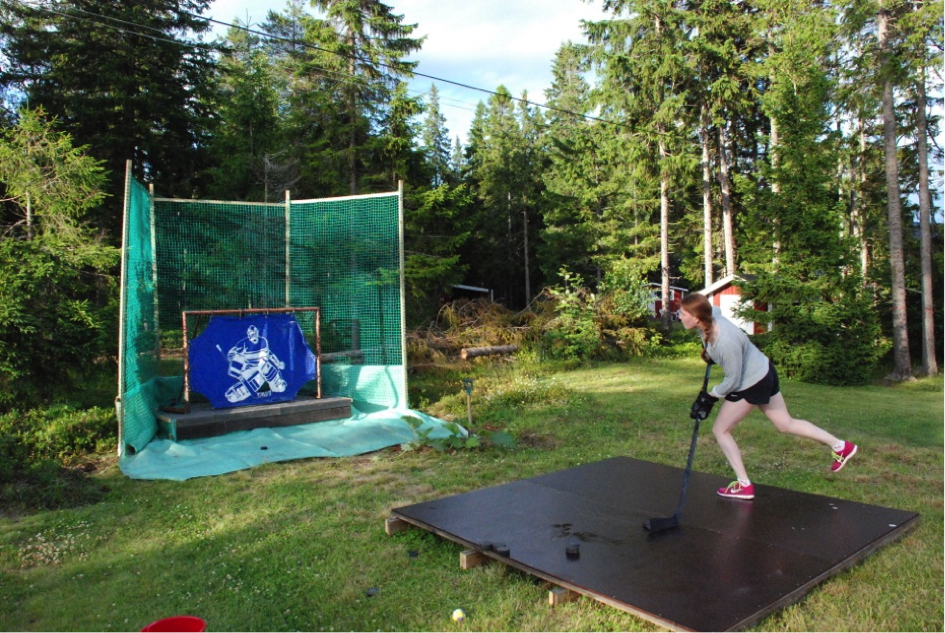
\includegraphics[width=\linewidth]{photos/the-incredible-shooting-ramp-my-mom-built-for-me.png}
  \caption{Exempel på skottrampsträning utomhus
  (\href{https://yalewomenshockey.wordpress.com/2013/07/18/ywih-summer-blog-hanna-astrom/}{YALE Womens Hockey's Blog}).
  \label{fig:skottramp}}
\end{figure}

Idrottsforskaren Johnny Nilsson har tillsammans med kollegor på Dalarna
University filmat skottrampsträningar (figur~\ref{fig:leksand}) och manuellt
analyserat resultatet för att få grundläggande statistiska mått vad gäller
träffbilder. Denna metod har visat sig mycket tidskrävande, till stor del
på grund av att hög precision är betydligt svårare att uppnå än vad det först
verkar, något som kan ses i figur~\ref{fig:skott}.

\begin{figure}[ht]
  \centering
  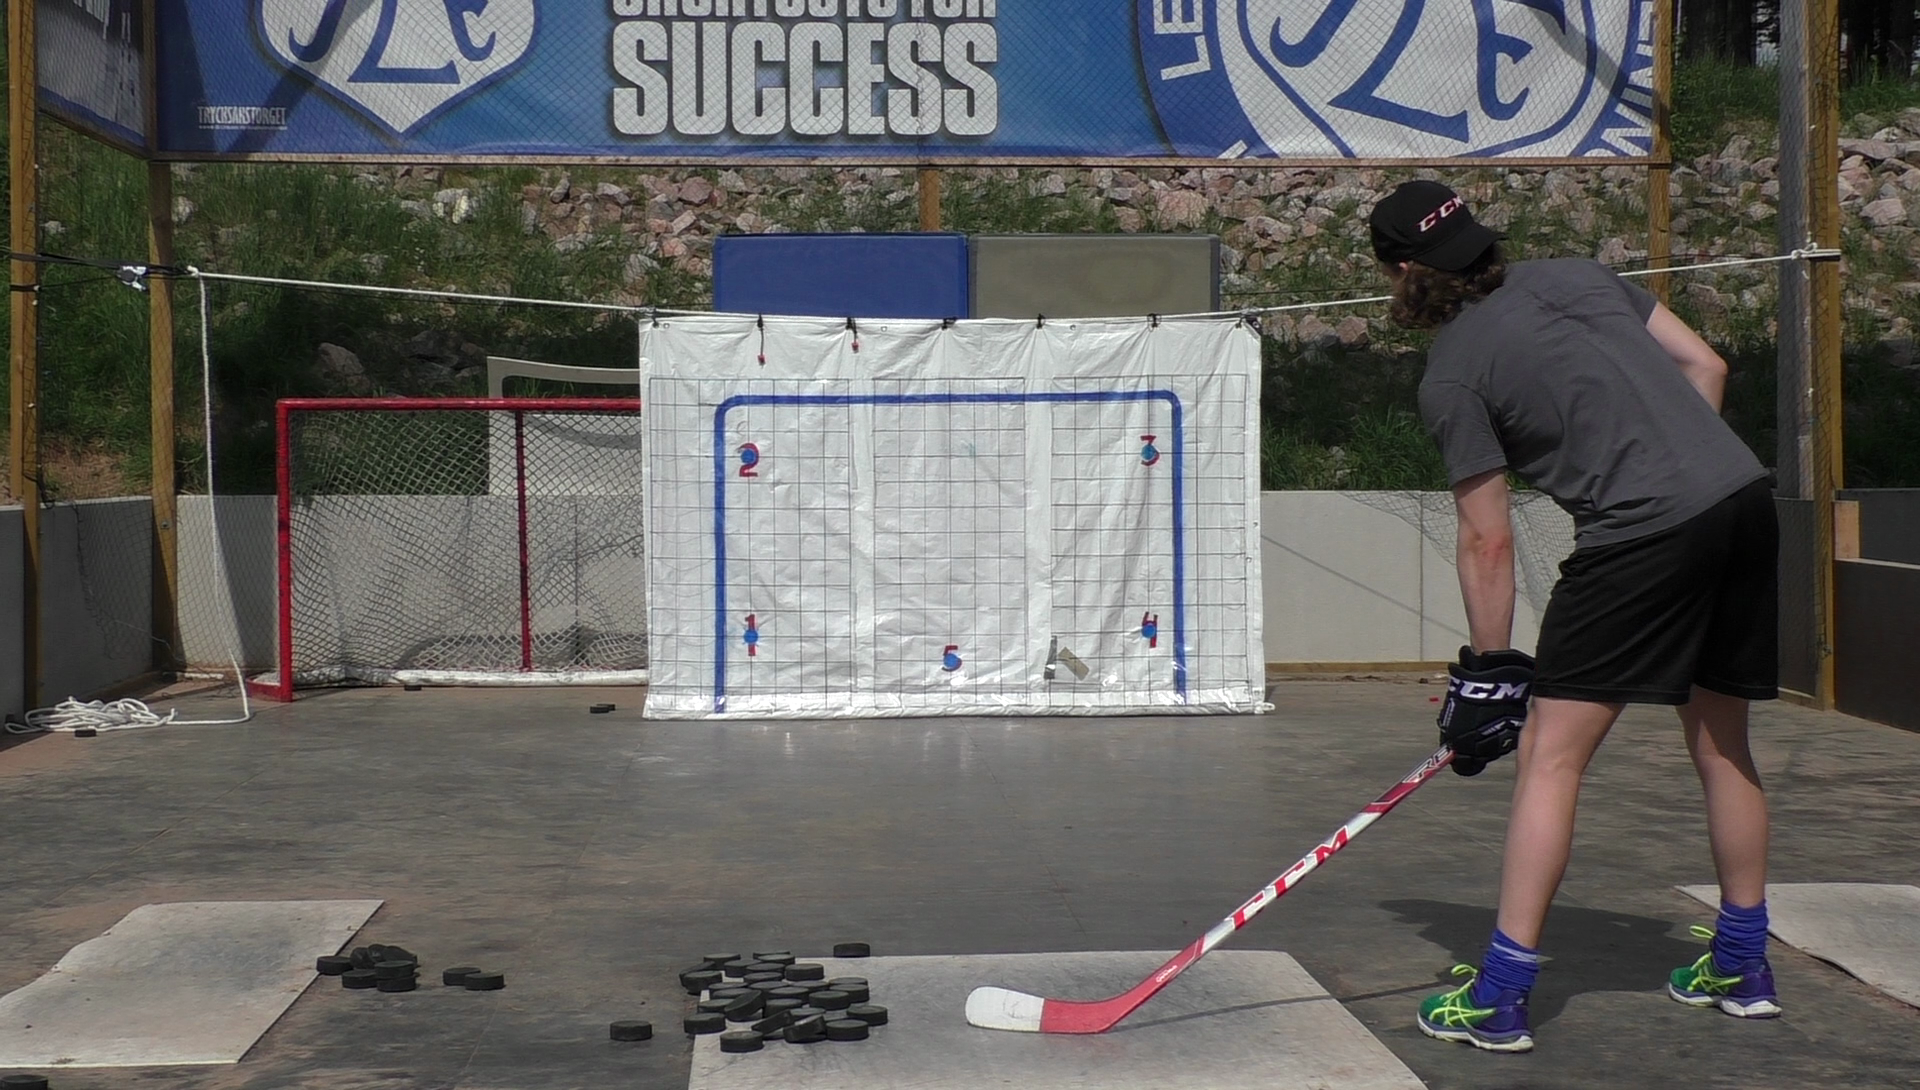
\includegraphics[width=\linewidth]{photos/skottrampstraning-leksands-if.png}
  \caption{Bildruta från videoinspelning av skottrampsträning. Duken är
    en prototyp, anpassad för manuell analys. Kamerans placering bakom
    spelaren är inte optimal för automatisk analys då spelaren och spelarens
    klubba ibland skymmer träffpunkten. För automatisk analys är det bättre
    att placera kameran på sidan framför spelaren, i en vinkel mot målet.
  \label{fig:leksand}}
\end{figure}

\begin{figure}[ht]
  \centering
  \begin{subfigure}[t]{0.24\textwidth}
    \centering
    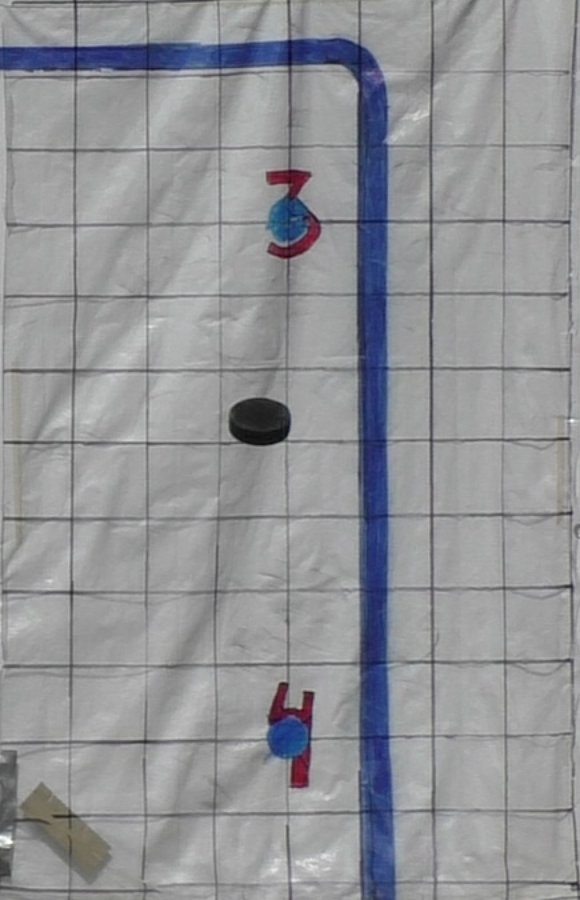
\includegraphics[width=\linewidth]{photos/skott1.png}
  \end{subfigure}%
  \hspace*{\fill}
  \begin{subfigure}[t]{0.24\textwidth}
    \centering
    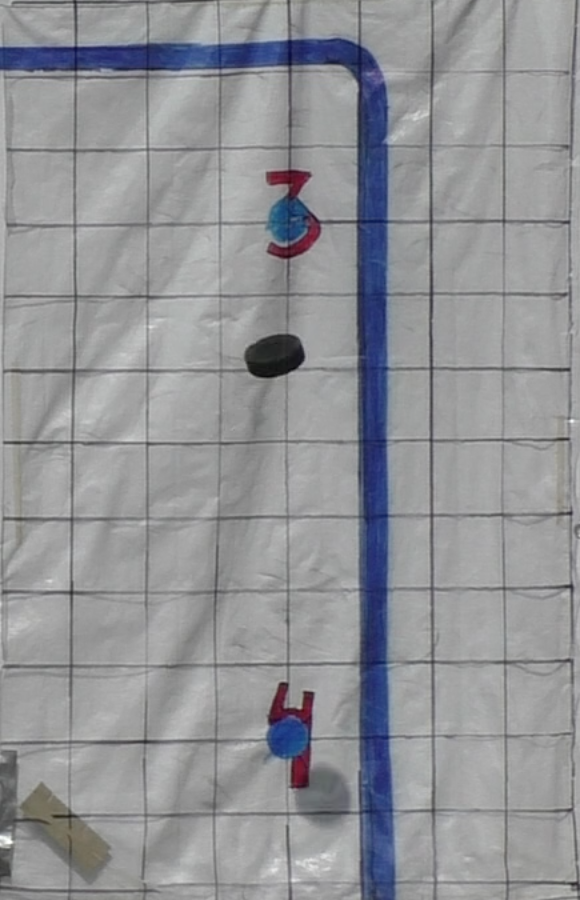
\includegraphics[width=\linewidth]{photos/skott2.png}
  \end{subfigure}%
  \hspace*{\fill}
  \begin{subfigure}[t]{0.24\textwidth}
    \centering
    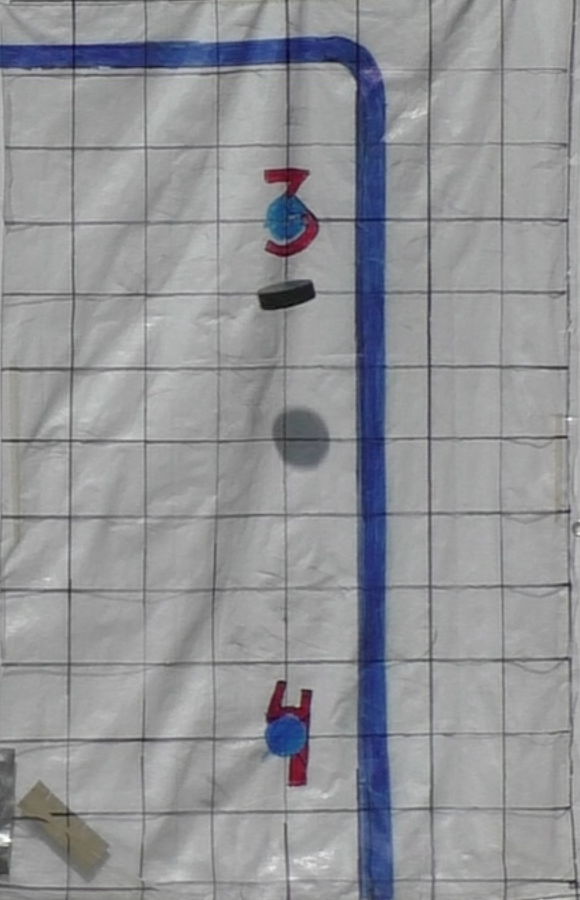
\includegraphics[width=\linewidth]{photos/skott3.png}
  \end{subfigure}%
  \hspace*{\fill}
  \begin{subfigure}[t]{0.24\textwidth}
    \centering
    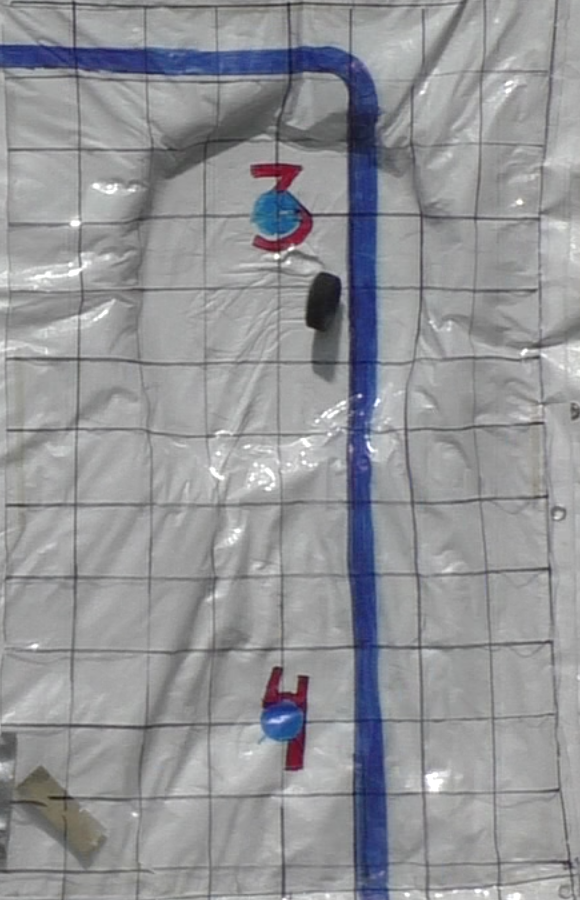
\includegraphics[width=\linewidth]{photos/skott4.png}
  \end{subfigure}%

  \caption{Även manuellt kan det vara svårt att avgöra exakt var pucken
    träffade duken. Det gäller att försöka uppskatta avståndet i centimeter
    till den målpunkt som spelaren försökt träffa, här nummer 3. Rutnätet,
    $10 \times 10$~cm är till för okulär kvantifiering av träffdata (utsnitt
    ur träningsserie, filmad med videokamera i 60 fps).\label{fig:skott}}
\end{figure}

Nilssons problem gav 2017 upphov till ett MVK-projekt på KTH och en
prototyp som visade att det bör vara möjligt att automatisera processen med
precision som närmar sig motsvarande manuell analys om filmer med hög
upplösning och hög frekvens används som källmaterial.

Ett av grundproblemen vad gäller att med precision avgöra en pucks träffpunkt
är att position och riktning måste bestämmas i tre dimensioner. Med ett
tänkt plan parallellt med målburens framsida, längs mållinjen, så är det
endast när en puck passerar planet (i rätt riktning\footnote{Puckar kan t.ex.
rulla ut eller träffa andra puckar inne i målburen och få dem att studsa
ut.}) som dess koordinat ska registreras. Om registrering sker framför eller
bakom planet så påverkas precisionen negativt.

\begin{figure}[ht]
  \centering
  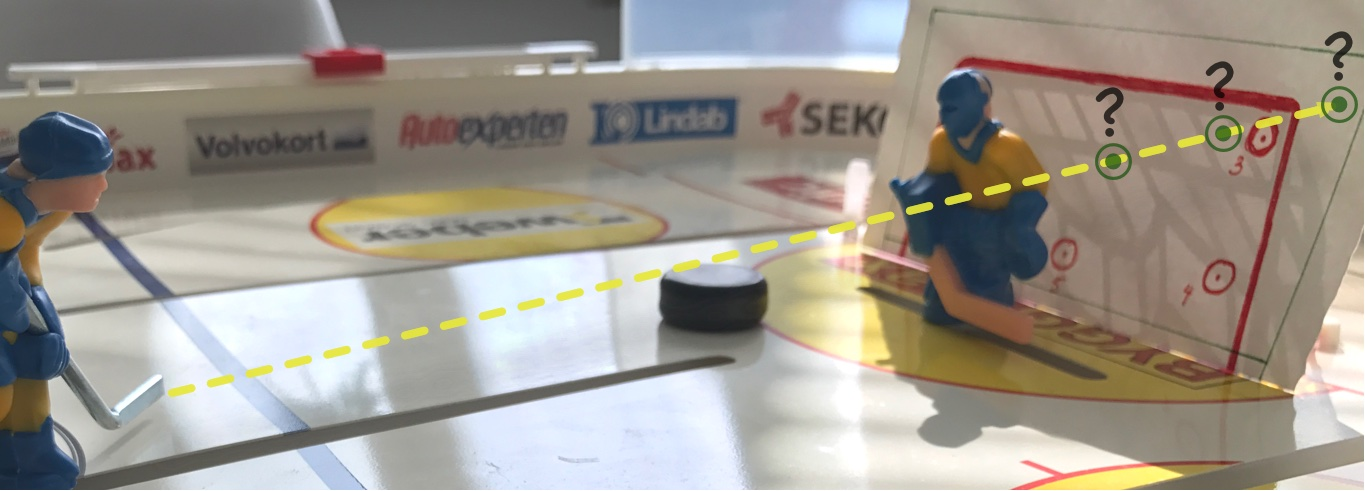
\includegraphics[width=\linewidth]{photos/3d-problem-two.jpg}
  \caption{I två dimensioner är det svårt att bestämma var pucken korsar
    planet längs mållinjen och målburens framsida.
  \label{fig:3d-problem2}}
\end{figure}

En vanlig kamera fångar bara två dimensioner och även om det ibland är möjligt
att återskapa tre dimensioner hos vissa objekt genom deras geometriska
egenskaper så låter sig detta inte göras med en hockeypuck som rör sig 30~m/s.
Med andra ord -- även om det skulle forskas fram en perfekt algoritm för att
följa en hockeypuck i två dimensioner så går det ändå inte att avgöra
\textit{exakt} när pucken passerar mållinjen\footnote{Givet att inte kameran
är riktad längs mållinjen men då går det inte längre att avgöra puckens
koordinat relativt målburens hörn.} (se figur~\ref{fig:3d-problem2}).

\begin{figure}[ht]
  \centering
  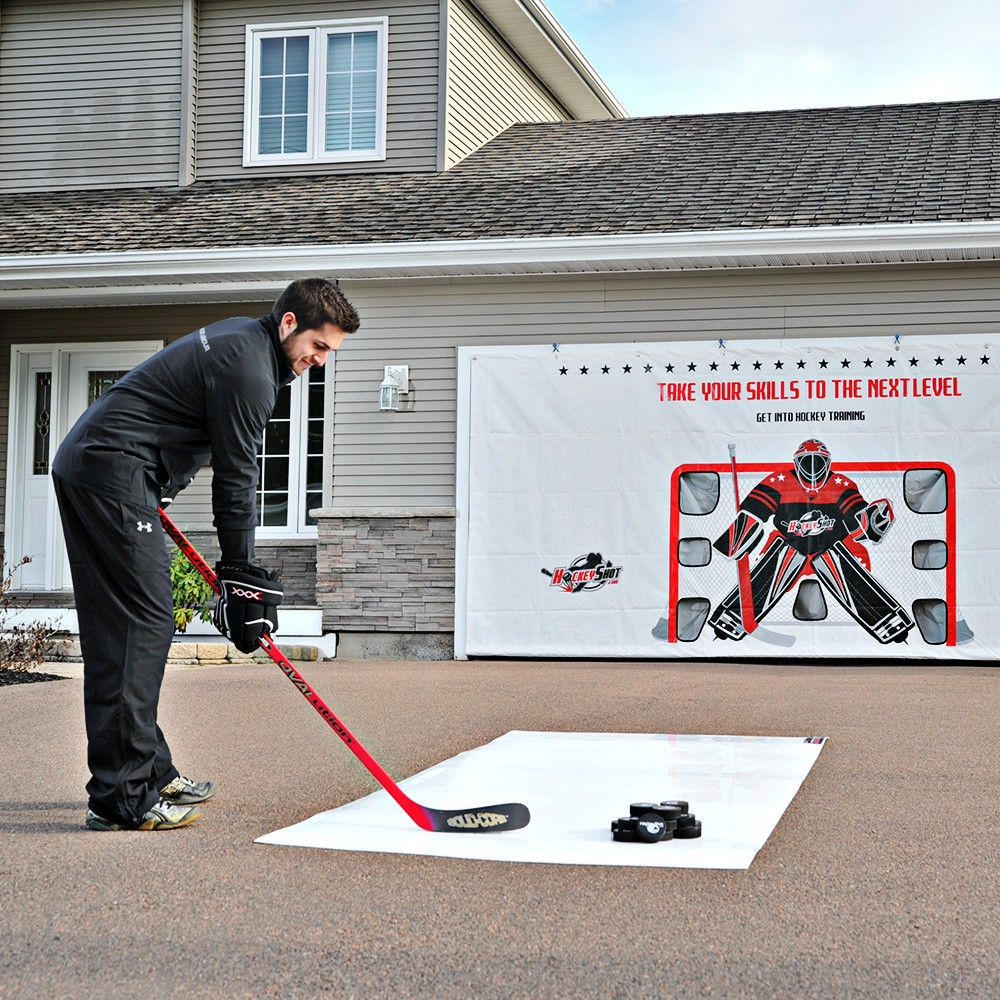
\includegraphics[width=\linewidth]{photos/shooting-tarp.jpg}
  \caption{Exempel på duk
  (\href{http://www.hockeyshot.se/HockeyShot-Extreme-Shooting-Tarp-p/target-tarp-032.htm}{hockeyshot.se}).
  \label{fig:duk}}
\end{figure}

Nilssons lösning är att låta pucken träffa en tålig duk som motsvarar planet
parallellt med mållinjen. En pragmatisk och kostnadseffektiv metod, väl
anpassad till att skottrampsträning ofta redan genomförs med hjälp av duk
(se figur~\ref{fig:skottramp} och~\ref{fig:duk}). Mycket övergripande skulle
analysen då kunna brytas ned i tre steg:

\begin{enumerate}
  \item \label{enum:step1} Hitta dukens koordinatsystem givet godtycklig
    kameravinkel.
  \item \label{enum:step2} Hitta bildrutan då pucken träffar duken.
  \item \label{enum:step3} Hitta puckens koordinater i denna bildruta utifrån
    ovanstående koordinatsystem.
\end{enumerate}

Alla tre steg har en avgörande påverkan på analysens kvalitet och är
intressanta problem i sig själva. Det här arbetet kommer fokusera på
steg~\ref{enum:step2} och eftersom det visuellt är lätt att se skillnaden
mellan när pucken bara färdas framför duken och när den verkligen träffar
(se figur~\ref{fig:skott} och figur~\ref{fig:hit-not-hit}) så verkar det
rimligt att någon form av datorseende skulle kunna användas för att
automatisera processen.
\begin{figure}[ht]
  \centering
  \begin{subfigure}[t]{\textwidth}
    \centering
    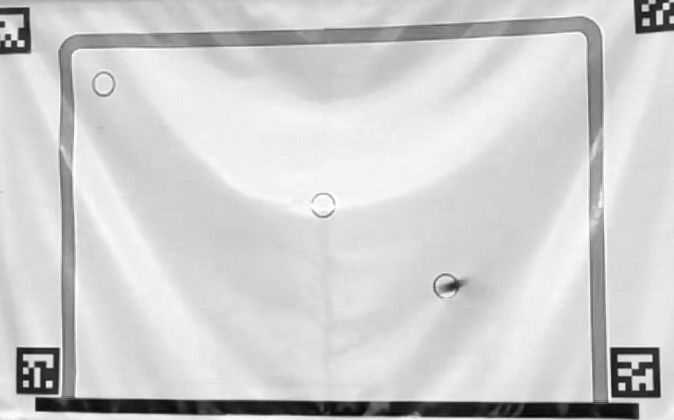
\includegraphics[width=\linewidth]{photos/canvas-not-hit.jpg}
  \end{subfigure}\\
  \begin{subfigure}[t]{\textwidth}
    \centering
    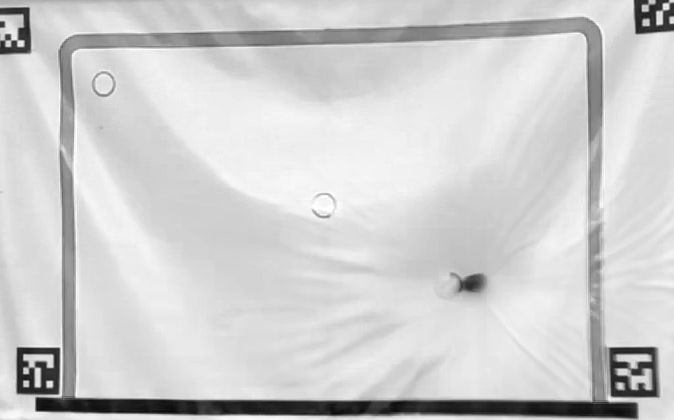
\includegraphics[width=\linewidth]{photos/canvas-hit.jpg}
  \end{subfigure}%
  \caption{Visuellt är oftast enkelt att skilja icke-träffar från
    träffar (utsnitt ur träningsserie, filmad med mobilkamera i
    120~fps.).\label{fig:hit-not-hit}}
\end{figure}
Det finns dock flera komplicerande faktorer, följande har t.ex.
observerats på filmer från skottrampsträning:
\begin{itemize}
  \item Allt som rör sig är inte pucken som träffar duken. Om inget annat så
    rör sig pucken framför duken innan den träffar men det är också troligt
    att duken inte helt slutat röra sig efter förra träffen (se t.ex. video
    [\cite{Nockert:2018a}]). Utomhus kan vind få duken att bölja. Inomhus kan
    vibrationer i golvet orsaka skakningsoskärpa (vilket innebär rörelse i
    hela bilden).
  \item Solljuset varierar över tid och skapar reflektioner i duken. Skuggor
    från träd, moln och fönsterbågar kan röra sig över duken. Humlor och löv
    kan flyga framför duken.
  \item Om pucken träffar ett hörn rör sig duken väldigt lite jämfört med en
    träff i mitten. Utan någon form av kalibrering är inte spannet känt och
    det är inte uppenbart hur det går att avgöra om en rörelse är tillräcklig
    för att motsvara en träff, speciellt som skottet helt kan ha missat duken.
  \item Form och storlek på en puck är inte visuellt konsistent under rörelse.
    I en viss betraktningsvinkel ser den ut som en cirkel, i andra vinklar som
    en ellips eller en tunn rektangel. Det är på så sätt svårt att definitivt
    avgöra om något är en puck eller inte. Hårda skott gör att pucken får
    rörelseoskärpa även med högre inspelningsfrekvenser.
  \item Det kan finnas fler än en puck i bild. Puckar blir framförallt
    liggande runt målet men de kan också glida eller rulla på marken många
    sekunder efter de träffat duken.
\end{itemize}

På grund av puckens form sker studsen mot duken inte kontrollerat och därför
är det viktigt att försöka identifiera en bildruta så nära tidpunkten då
pucken först träffar duken.

Baserat på ovanstående verkar initialt problemet kunna modelleras som ett
(intressant) rörelsedetektionsproblem där solljus, svängningar i duken och
puckens rörelse innan träff tillhör bakgrundsmodellen och träffbilden tillhör
förgrund. Rörelsedetektion verkar dessvärre vara ett relativt svårt område
inom datorseende och det är inte triviala fall som måste hanteras här.
Framförallt verkar inte syftet vara att tillförlitligt hitta \textit{tidigaste}
bildrutan där rörelse upptäcks och det är inte uppenbart hur en lösning
med den här metoden skulle kunna vara till hjälp i letandet bakåt efter
bildrutan av intresse.

Problemet verkar också kunna modelleras som ett binärt klassificeringsproblem
där bildrutor antingen visar en duk som ännu inte träffats av pucken eller
en duk som precis träffats av pucken. Ett faltningsneuronnät skulle
kunna tränas på dessa två situationer och ge en modell som svarar mot
sannolikheten att en bild är en träff eller en icke-träff.

Givet att varje skott är tidsmässigt avgränsat från andra skott så är
hypotesen att bildrutorna i princip skulle kunna behandlas sekvensiellt och
första bildrutan som modellen klassificerar som träff vara bildrutan i
vilken puckens position ska bestämmas. Hypotesen är också att bilderna
i \textit{båda} kategorierna kommer variera i termer av solljus,
duksvängningar, puckar i rörelse, etc. att neuronnätet kommer bortse från
detta i klassificeringen.


\section*{Syfte}
Undersöka hur väl faltningsneuronnät svarar mot bestämning av tidpunkt för
träff av hockeypuck mot målduk (steg~\ref{enum:step2} ovan) jämfört med
manuellt identifierade tidpunkter. Detta inkluderar att undersöka i vilken
grad modellen blir invariant mot förändringar som visuellt skiljer sig från de
orsakade av att en puck träffar duken.

Kan tidsstämplingen göras mer tillförlitlig under verkliga omständigheter bör
kvaliteten på den automatiska analysen öka avsevärt. Framför allt finns en
önskan om att minimera antalet identifikationer med stor tidsavvikelse, något
som kan leda till att träffen placeras långt (meter snarare än centimeter)
ifrån den faktiska träffpunkten.

Målet är inte en perfekt algoritm utan en algoritm med kända prestanda
gentemot noggrann manuell analys, samt statistisk referensdata så att
förbättrade algoritmer kan jämföras med resultaten från den här studien i
framtiden. Syftet, i förlängningen, är att möjliggöra forskning inom
ishockeyträning baserad på stora mängder träningsdata över tid samt bädda för
produkter för systematisk precisionsträning med hjälp av skottramp.


\section*{Metod och teknik}
Arbetet är av utforskande karaktär och är tänkt att utmynna i en algoritm
med kvantifierad prestanda. Arbetsmomenten består av datainsamling såväl
som teoretiska och praktiska undersökningar:
\begin{itemize}
  \item skapa referensdata genom att spela in filmer från skottrampsträning,
    noggrant manuellt analysera dem vad gäller tidpunkter för träff samt
    klassificera bildrutor som antingen träffar eller icke-träffar.
  \item hjälpa till att ta fram en duk som underlättar automatisk analys av
    skottrampsträning,
  \item med hjälp av Python, Tensorflow, Keras och OpenCV undersöka
    skapande av faltningsneuronnät för binär klassificering av bilder
    från skottrampsträning.
  \item sätta samman metoder för bildbehandling och bildanalys med
    neuronnät till en algoritm som kan valideras praktiskt genom applikation
    på referensfilmer och jämföras med tidpunkter från manuell analys med
    hög temporal och spatial upplösning (''gold standard''),
\end{itemize}


\section*{Avgränsning}
Det är inom ramarna för detta arbete inte rimligt att hysa någon förhoppning
om att skapa en perfekt algoritm. Därför kommer i första hand högnivåmetoder
som redan finns implementerade i Keras och OpenCV användas snarare än att
bygga eget på låg nivå.

Arbetet utförs med antagandet att steg~\ref{enum:step1} hanteras så nära
perfekt som möjligt och att steg~\ref{enum:step3} är relativt enkelt givet
att bildrutan för träff är identifierad. Det antas med andra ord att
steg~\ref{enum:step3} enbart behöver använda en tidpunkt/bildruta som indata
för att bestämma puckens position. På så sätt behöver beslut i det här
arbetet inte beakta eventuell intern nytta i de andra stegen.


\pagebreak
\section*{Planering/tidplan}
Kursen kommer läsas i halvfart HT18. Kursen i vetenskaplighet som ingår
i uppsatsarbetet slutfördes under VT18. Uppsatsen skrivs på engelska.

\subsection*{September}
\begin{itemize}
  \item Övergripande undersöka domänen för faltningsneuronnät och binär
    klassificering. Teori, metoder, problem och möjligheter i relation till
    ovanstående. Samla relevanta källor.
  \item Undersöka domänen kring skottrampsträning för att i sin tur, i
    samarbete med Johnny Nilsson, ta fram en målduk och metod för mätning
    som väger in den algoritmiska komplexiteten på en datorseendelösning
    (mycket av det är redan gjort under sommaren 2018).
  \item Skriva på uppsatsens bakgrund.
  \item Använda mobilkamera för att spela in filmer för att få initial
    tränings"~, validerings"~ och testdata samt utvärdera utformning på
    målduken (mobil är den tänkta enheten för framtida träningsprodukter
    och borde också kunna vara ett enkelt och tillgängligt forskningsverktyg).
  \item Analysera filmer manuellt och klassificera bildrutor.
\end{itemize}

\subsection*{Oktober}
\begin{itemize}
  \item Skriva syfte och begränsningar.
  \item Vid behov justera duk och mätmetod baserat på resultatet så här långt.
    Spela in nya filmer med skickliga hockeyspelare, etablera kompletterande
    referensdatamängd. Jämföra med de tidigare resultaten.
  \item Låna duk av Nilsson för att kunna spela in filmer under naturliga
    förhållanden med syfte att etablera referensdata vid olika väder, olika
    tider på dygnet, etc. (möjligen går det att använda filmer inspelade
    augusti 2018).
  \item Undersöka angreppsättet från det tidigare MVK-projektet, dels med
    avseende på analysmetod och dels med avseende på kvalitativt mått för
    testning som väger in både koordinatförskjutning och tidsförskjutning
    gentemot referensdata.
  \item Utgå från grundläggande, generella metoder för binär klassificering
    tillsammans med Python och Keras, för att få en bättre bild av vad som
    måste hanteras specifikt för domänen.
  \item Skriva på metoddel och avhandlingsdel.
\end{itemize}

\subsection*{November}
\begin{itemize}
  \item Fortsätta undersöka metoder för neuronnät med hjälp av referensdata
    (inspelade filmerna från september och oktober, samt filmer inspelade
    vid tidigare tillfällen), speciellt i avseende på fall som
    uppkommer under naturliga förhållanden.
  \item Komplett algoritm med neuronnät som central komponent.
  \item Sammanställa resultat i form av en jämförelse med manuellt
    analyserade filmer, både vad gäller sammantagen avvikelse och vad
    gäller utliggare och extremfall.
  \item Skriva metoddel, avhandlingsdel, diskussionsdel och slutsatser.
\end{itemize}

\subsection*{December}
\begin{itemize}
  \item Skriva avslutning och abstract.
  \item Färdigställa uppsats.
\end{itemize}

\subsection*{Januari}
\begin{itemize}
  \item Presentation innan VT19 börjar.
\end{itemize}

\printbibliography{}
\end{document}
